	\section{Equação do 1° grau}

    \noindent
	\textbf{Definição:} Uma equação linear em $x$ pode ser escrita da seguinte forma:
        \begin{tcolorbox}[colback=white,colframe=minha_cor,coltitle=black,title=Definição] 
        \[
        ax+b=0,
        \]
        \[
		\text{em que a, b}  \in \mathbb{R}\text{ e } a \neq 0
        \]
        \end{tcolorbox}
    O objetivo de uma equação do 1° grau é encontrar o valor que satisfaz a igualdade.

    \noindent
	\textbf{Exercícios Resolvidos}
	\begin{enumerate}
		\item Resolver a equação em $\mathbb{R}$.
		\begin{enumerate}
			\item $23x-16=14-17x$ \\
			Fazendo:\\
			$y=23x-16$\\
			$y=14-17x$\\ 
   \begin{center}
        \begin{tikzpicture}
            \begin{axis}[
            width=0.8\textwidth,
            xlabel=$x$,
            ylabel=$y$,
            axis lines=middle,
            xmin=-2,
            xmax=2,
            ymin=-20,
            ymax=20,
            xtick={-2,-1,...,2},
            ytick={-20,-15,...,20},
            enlargelimits,
            ticks=both,
            %tick label style={font=\small}, % para diminuir o tamanho de fonte
            tick label style={font=\footnotesize}, % outra opção de tamanho de fonte
            % tick label style={font=\tiny} % é a menor fonte q tem
            after end axis/.code={
            \draw (axis cs:0,\pgfkeysvalueof{/pgfplots/ymin}) -- (axis cs:0,\pgfkeysvalueof{/pgfplots/ymax});
            \draw (axis cs:\pgfkeysvalueof{/pgfplots/xmin},0) -- (axis cs:\pgfkeysvalueof{/pgfplots/xmax},0);
            \node[black, above right] at (axis cs:1,5) {$y =23x-16 $};
            \node[black, below right] at (axis cs:0.7,-15) {$y =14-17x$};
            }
            ]
            \addplot[domain=-2:4, blue, samples=100] {23*x-16};
            \addplot[domain=-2:4, Green, samples=100] {14-17*x};
            \end{axis}
        \end{tikzpicture}
    \end{center}
    
			Em seguida, faz-se:
			\[
			23x-16=14-17x
			\]
			Soma-se 17$x$ e 16 de ambos os lados da igualdade
			\[
			23x-16 +17x +16=14-17x+17x +16
			\]
			\[
			40x = 30
			\]
			Divide-se ambos os lados da igualdade por 40
			\[
			\dfrac{40x}{40} = \dfrac{30}{40}
			\]
			\[
			x=\dfrac{3}{4}
			\]
			Assim, o conjunto solução do problema é
			\[
			S=\left\{ \dfrac{3}{4} \right\}
			\]
			%%%%%%%%%%%%%%%%%%%%%%%%%%%%%%%%%%%%%%
			\item $10y-5(1+y)=3(2y-2)-20$\\
			Fazendo:\\
			$y=10x-5(1+x)$\\
			$y=3(2x-2)-20$\\   
   
			%%%%%%%%%%%%%% gráfico %%%%%%%%%%%%%%%
    \begin{center}
            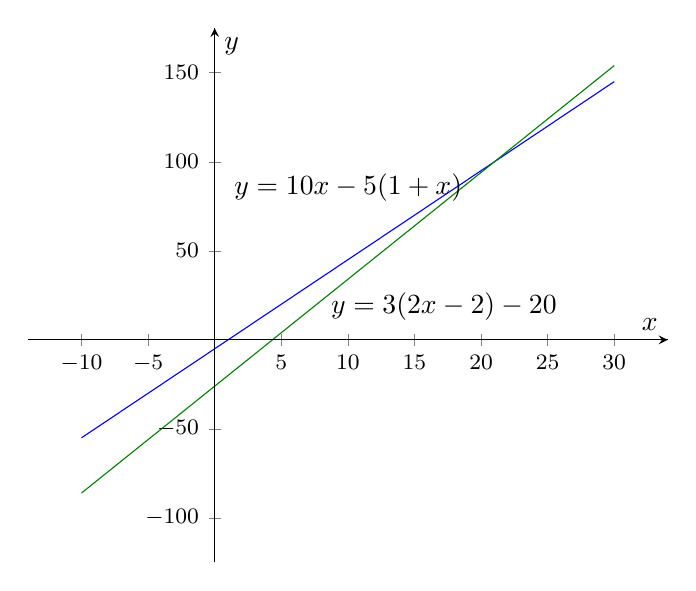
\begin{tikzpicture}
            \begin{axis}[
            width=0.8\textwidth,
            xlabel=$x$,
            ylabel=$y$,
            axis lines=middle,
            xmin=-10,
            xmax=30,
            ymin=-100,
            ymax=150,
            xtick={-10,-5,...,30},
            ytick={-100,-50,...,150},
            enlargelimits,
            ticks=both,
            %tick label style={font=\small}, % para diminuir o tamanho de fonte
            tick label style={font=\footnotesize}, % outra opção de tamanho de fonte
            % tick label style={font=\tiny} % é a menor fonte q tem
            after end axis/.code={
            \draw (axis cs:0,\pgfkeysvalueof{/pgfplots/ymin}) -- (axis cs:0,\pgfkeysvalueof{/pgfplots/ymax});
            \draw (axis cs:\pgfkeysvalueof{/pgfplots/xmin},0) -- (axis cs:\pgfkeysvalueof{/pgfplots/xmax},0);
            \node[black, above right] at (axis cs:0.75,72) {$y=10x-5(1+x)$};
            \node[black, below right] at (axis cs:8,32) {$y=3(2x-2)-20$};
            }
            ]
            \addplot[domain=-10:30, blue, samples=100] {5*x - 5};
            \addplot[domain=-10:30, Green, samples=100] {6*x - 26};
            \end{axis}
        \end{tikzpicture}
    \end{center}
            %%%%%%%%%%%%%%%%%%%%%%%%%%%%%%%%%%%%%%
            
			Em seguida, faz-se:
			\[
			10y-5(1+y)=3(2y-2)-20
			\]
			Aplicando a distributiva
			\[
			10y-5-5y=6y-6-20
			\]
			Soma-se $-6y$ e 5 de ambos os lados da igualdade
			\[
			5y-5-6y+5=6y-26-6y+5
			\]
			\[
			-y = -21
			\]
			\[
			\cdot (-1) -y = \cdot (-1) -21
			\]
			\[
			y = 21
			\]
			\[
			S=\left\{ 21 \right\}
			\]
			%%%%%%%%%%%%%%%%%%%%%%%%%%%%%%%%%%%%%%
			\item $x(x+4)+x(x+2) = 2x^2+12$
			Fazendo a distributiva, obtém-se:\\
			\[
			2x^2 + 6x = 2x^2 + 12
			\]  
			Plotando os gráficos das equações do 2ºgrau, obtém-se:\\
   
            %%%%%%%%%%%%%%%%%%%%%%%%%%%%%%%%%%%%%%
    \begin{center}
            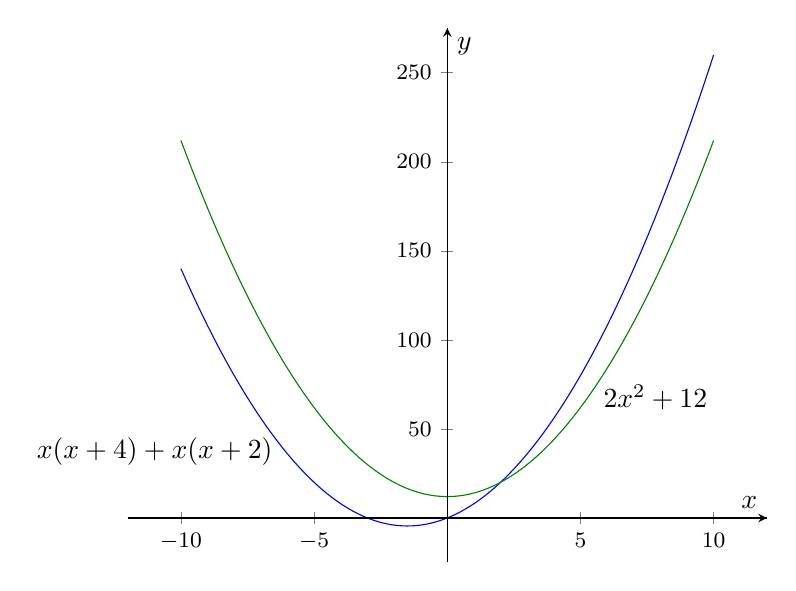
\begin{tikzpicture}
            \begin{axis}[
            width=0.8\textwidth,
            xlabel=$x$,
            ylabel=$y$,
            axis lines=middle,
            xmin=-10,
            xmax=10,
            ymin=0,
            ymax=250,
            xtick={-10,-5,...,10},
            ytick={0,50,...,250},
            enlargelimits,
            ticks=both,
            %tick label style={font=\small}, % para diminuir o tamanho de fonte
            tick label style={font=\footnotesize}, % outra opção de tamanho de fonte
            % tick label style={font=\tiny} % é a menor fonte q tem
            after end axis/.code={
            \draw (axis cs:0,\pgfkeysvalueof{/pgfplots/ymin}) -- (axis cs:0,\pgfkeysvalueof{/pgfplots/ymax});
            \draw (axis cs:\pgfkeysvalueof{/pgfplots/xmin},0) -- (axis cs:\pgfkeysvalueof{/pgfplots/xmax},0);
            \node[black, above left] at (axis cs:-6.2,24) {$x(x+4)+x(x+2)$};
            \node[black, below right] at (axis cs:5.5,80) {$2x^2+12$};
            }
            ]
            \addplot[domain=-10:10, blue, samples=100] {2*x^2 + 6*x};
            \addplot[domain=-10:10, Green, samples=100] {2*x^2 + 12};
            \end{axis}
        \end{tikzpicture}
    \end{center}
            %%%%%%%%%%%%%%%%%%%%%%%%%%%%%%%%%%%%%%
			
			Soma-se $2x^2$ de ambos os lados da igualdade
			\[
			2x^2 + 6x  -2x^2= 2x^2 + 12 -2x^2
			\]
			\[
			6x = 12
			\]
			Divide-se ambos os lados da igualdade por 6
			\[
			\dfrac{6x}{6} = \dfrac{12}{6}
			\]
			\[
			x=2
			\]
			Assim, o conjunto solução do problema é
			\[
			S=\left\{ 2 \right\}
			\]
			%%%%%%%%%%%%%%%%%%%%%%%%%%%%%%%%%%%%%%
			\item $\dfrac{x-5}{10} + \dfrac{1-2x}{5} = \dfrac{3-x}{4}$\\
			
			Encontrando o MMC dos denominadores(10, 5), obtém-se:\\
			\[
			\dfrac{1 \cdot (x-5) + 2 \cdot (1-2x)}{10} = \dfrac{3-x}{4}
			\]  
			Aplicando a distributiva, obtém-se:
			\[
			\dfrac{x-5+2-4x}{10} = \dfrac{3-x}{4} 
			\]
			\[
			\dfrac{-3x-3}{10} = \dfrac{3-x}{4} 
			\]
			Plotando o gráfico, obtém-se:\\

            %%%%%%%%%%%%%%%%%%%%%%%%%%%%%%%%%%%%%%
    \begin{center}
            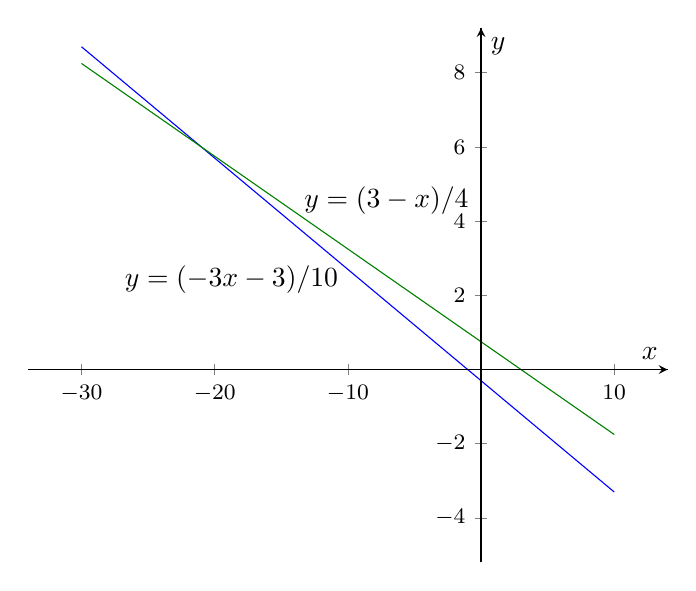
\begin{tikzpicture}
            \begin{axis}[
            width=0.8\textwidth,
            xlabel=$x$,
            ylabel=$y$,
            axis lines=middle,
            xmin=-30,
            xmax=10,
            ymin=-4,
            ymax=8,
            xtick={-30,-20,...,10},
            ytick={-4,-2,...,8},
            enlargelimits,
            ticks=both,
            %tick label style={font=\small}, % para diminuir o tamanho de fonte
            tick label style={font=\footnotesize}, % outra opção de tamanho de fonte
            % tick label style={font=\tiny} % é a menor fonte q tem
            after end axis/.code={
            \draw (axis cs:0,\pgfkeysvalueof{/pgfplots/ymin}) -- (axis cs:0,\pgfkeysvalueof{/pgfplots/ymax});
            \draw (axis cs:\pgfkeysvalueof{/pgfplots/xmin},0) -- (axis cs:\pgfkeysvalueof{/pgfplots/xmax},0);
            \node[black, above left] at (axis cs:-10,1.8) {$y=(-3x-3)/10$};
            \node[black, below right] at (axis cs:-14,5.2) {$y=(3-x)/4$};
            }
            ]
            \addplot[domain=-30:10, blue, samples=100] {(-3*x-3)/10};
            \addplot[domain=-30:10, Green, samples=100] {(3-x)/4};
            \end{axis}
            \end{tikzpicture}

    \end{center}
            %%%%%%%%%%%%%%%%%%%%%%%%%%%%%%%%%%%%%%
            
			\[
			\dfrac{-3x-3}{10} \cdot (10) \cdot (4)= \dfrac{3-x}{4} \cdot (10) \cdot (4)
			\]
			\[
			4(-3x-3)=10(3-x)
			\]
			Aplicando a distributiva, obtém-se:
			\[
			-12x-12 = 30-10x
			\]
			Soma-se $10x$ e 12 de ambos os lados da igualdade
			\[
			-12x-12 +10x +12= 30-10x +10x +12
			\]
			\[
			-2x = 42
			\]
			Divide-se ambos os lados da igualdade por -2
			\[
			\dfrac{-2x}{-2} = \dfrac{42}{-2}
			\]
			\[
			x=-21
			\]
			Assim, o conjunto solução do problema é
			\[
			S=\left\{ -21 \right\}
			\]
			%%%%%%%%%%%%%%%%%%%%%%%%%%%%%%%%%%%%%%
			\item $\dfrac{5}{x}-2 = \dfrac{1}{4}$\\
			
			Observa-se que $x = 0$ não é possível\\
			Plotando o gráfico, temos:\\
   
			%%%%%%%%%%%%%%%%%%%%%%%%%%%%%%%%%%%%%%
   \begin{center}
            \begin{tikzpicture}
            \begin{axis}[
            width=0.8\textwidth,
            xlabel=$x$,
            ylabel=$y$,
            axis lines=middle,
            xmin=0,
            xmax=4,
            ymin=-3,
            ymax=6,
            xtick={-1,0,...,4},
            ytick={-3,-2,...,6},
            enlargelimits,
            ticks=both,
            %tick label style={font=\small}, % para diminuir o tamanho de fonte
            tick label style={font=\footnotesize}, % outra opção de tamanho de fonte
            % tick label style={font=\tiny} % é a menor fonte q tem
            after end axis/.code={
            \node[black, above right] at (axis cs:0.9,4) {$y=(5/x)-2$};
            \node[black, below right] at (axis cs:0.3,1.1) {$y=1/4$};
            }
            ]
            \addplot[domain=0:4, blue, samples=100] {5/x-2};
            \addplot[domain=-1:4, Green, samples=100] {1/4};
            \end{axis}
            \end{tikzpicture}
    \end{center}
            %%%%%%%%%%%%%%%%%%%%%%%%%%%%%%%%%%%%%%
			
			Soma-se $2$ de ambos os lados da igualdade
			\[
			\dfrac{5}{x}-2 {+2} = \dfrac{1}{4} {+2}
			\]
			\[
			\dfrac{5}{x} = \dfrac{9}{4}
			\]
			Desde que $x \neq 0$, multiplica-se ambos os lados da igualdade por $x$
			\[
			\dfrac{5}{x} \cdot (x)  = \dfrac{9}{4} \cdot (x)
			\]
			\[
			5= \dfrac{9}{4}\; x
			\]
			em seguida, multiplica-se os dois lados da igualdade pelo inverso de $\dfrac{9}{4}$, ou seja, por $\dfrac{4}{9}$
			\[
			5\; \cdot \left(\dfrac{4}{9}\right)= \dfrac{9}{4}\; x \;\cdot \left(\dfrac{4}{9}\right)
			\]
			\[
			x = \dfrac{20}{9}
			\]
			Assim, o conjunto solução do problema é
			\[
			S=\left\{ \dfrac{20}{9} \right\}
			\]
		\end{enumerate}

		\item Encontre $a_1$ e $a_2$ que satisfazem a equação.\\
		$\dfrac{2x-1}{x^2-5x+6} = \dfrac{a_1}{x-2}+\dfrac{a_2}{x-3}$\\
   
			Fazendo o MMC em os denominadores, $(x-2)(x-3)$, temos
			\[
			\dfrac{2x-1}{x^2-5x+6} = \dfrac{a_1(x-3)+a_2(x-2)}{(x-2)(x-3)}
			\]
			\[
			\dfrac{2x-1}{x^2-5x+6} = \dfrac{a_1 x-3a_1+a_2 x-2a_2}{x^2-5x+6}
			\]
			\[
			2x-1 = (a_1+a_2)x-(3a_1+2a_2)
			\]
   
			Assim, temos que resolver o sistema de equações
   
			\begin{equation*}
				\ \begin{cases}
					a_1+a_2 = 2 \;\; (i) \\
					3a_1+2a_2 = 1 \;\; (ii)
				\end{cases}
			\end{equation*}
			De  (i) temos $a_1 = 2 - a_2$, que substituindo em  (ii) fica:
			
			\[ 
            3(2-a_2)+2a_2 = 1 \Longrightarrow 6-3a_2+2a_2=1 
            \]
			\[ 
            \text{em (i)}\Longrightarrow 6-a_2=1 \Longrightarrow a_2 = 5
            \]
            
			Logo, voltando $a_1 = 2-a_2 = 2-5 \Longrightarrow a_1 = -3$ \\
			Portanto, a igualdade é satisfeita quando $a_1 = -3$ e $a_2 = 5$  \\
			\begin{center}
				\fbox{
					$\dfrac{2x-1}{x^2-5x+6} = \dfrac{-3}{x-2}+\dfrac{5}{x-3}$
				}
			\end{center}
	\end{enumerate}
	
	\section{Inequação do 1°grau}

    \noindent
	\textbf{Notação}
	\begin{itemize}
		\item {\Large <} :\;menor que;
		\item {\Large >} :\;maior que;
		\item {\Large $\le$} :\;menor que ou igual a;
		\item {\Large $\ge$} :\;maior que ou igual a.
	\end{itemize}

    \noindent
	\textbf{Definição}: Uma inequação linear em $x$ pode ser escrita das seguintes formas:

    \begin{tcolorbox}[colback=white,colframe=minha_cor,coltitle=black,title=Definição] 
        \begin{center}
        \begin{minipage}{0.6\textwidth}
        \[
        ax+b < 0, \;\; ax+b > 0, \;\; ax+b \le 0, \;\; ax+b \ge 0,
        \]
        $\text{em que }a, b \in \mathbb{R} \text{ e } a \neq 0.$
        \end{minipage}
        \end{center}
    \end{tcolorbox}
    
	

    \noindent
	\textbf{Propriedades}:
	Sejam $u$,$v$,$w$ e $z$ números reais, variáveis ou expressões algébricas, e $c$ uma constante real.
	\begin{itemize}
		\item \textbf{Transitiva}.\\
            Se  $u < v$ e $v < w$, então $u < w$.
		\item \textbf{Aditiva}. 
            \begin{description}
                \item[(i)]  Se  $u < v$, então $u + w < v +w$.
		      \item[(ii)] Se  $u < v$ e $w < z$, então $u + w < v +z$.
            \end{description}
		\item \textbf{Multiplicativa}. 
            \begin{description}
                \item[(i)]  Se  $u < v$ e $c > 0$, então $uc < vc$.
		      \item[(ii)] Se  $u < v$ e $c < 0$, então $uv > vc$.
            \end{description}
	\end{itemize}

    \noindent
	\textbf{Exercícios resolvidos}

%%% Aqui começa o exerc. 3 - Faltm os itens e), f), ..., i) %%%
	\begin{enumerate}
	   \item Resolva as inequações do primeiro grau:
            \begin{enumerate} 
			\item $2x - 8 > 0$\\
			Com o objetivo de isolar a variável $x$, soma-se $8$ nos dois lados da desigualdade
			\[ 
            2x - 8 +8 > 0 +8 
            \]
			\[ 
            2x > 8
            \]
			Em seguida, divide-se ambos lados por 2
			\[ 
            \dfrac{2x}{2}  > \dfrac{8}{2}  
            \]
			\[ 
            x > 4 
            \]
			Assim, o conjunto solução é
			\[
			S=\left\{ x \in \mathbb{R} \mid x >4 \right\} = (+4, +\infty) = \;]+4, +\infty[ 
			\]
			%%%%%%%%%%%%%%%%%%%%%%%%%%%%%%%%%%%%%%%%%%
			\item $3 + 7x < 8x + 9$\\
			Com o objetivo de isolar a variável $x$, subtrai-se $8x$ e $3$ nos dois lados da desigualdade
			\[ 
            3 + 7x-8x -3 < 8x + 9 -8x -3 
            \]
			\[ 
            -x < 6
            \]
			Em seguida, multiplica-se ambos lados por $-1$
			\[ 
            -x \;  \cdot (-1) \;  > \; 6 \;  \cdot (-1)
            \]
			\[ 
            x > -6
            \]
			Assim, o conjunto solução é
			\[
			S=\left\{ x \in \mathbb{R} \mid x > -6 \right\} = (-6, +\infty) = \; ]-6, +\infty[ 
			\]
			%%%%%%%%%%%%%%%%%%%%%%%%%%%%%%%%%%%%%%%%%%
			\item $\dfrac{x}{5} \le \dfrac{3}{4}$\\
			
			Com o objetivo de isolar a variável $x$, multiplica-se ambos lados da desigualdade por 5
			\[ 
            \dfrac{x}{5} \;  (\cdot \; 5) \le \dfrac{3}{4} \;  (\cdot \; 5)
            \]
			\[ 
            x \le \dfrac{15}{4}
            \]
			Assim, o conjunto solução é
			\[
			S=\left\{ x \in \mathbb{R} \mid x \le \dfrac{15}{4} \right\} = \left(-\infty,\dfrac{15}{4}\right] = \; \left]-\infty, \dfrac{15}{4}\right]
			\]
			%%%%%%%%%%%%%%%%%%%%%%%%%%%%%%%%%%%%%%%%%%
			\item $2x - 5 < \dfrac{1}{3}+\dfrac{3x}{4}+\dfrac{1-x}{3}$\\
			Com o objetivo de isolar a variável $x$, subtrai-se $\dfrac{1}{3}$ e soma-se $\dfrac{x}{3}$ e $5$ nos dois lados da desigualdade
			\[
			2x - \dfrac{3x}{4} < \dfrac{1}{3} + \dfrac{1}{3} - \dfrac{x}{3} + 5
			\]
			\[ 
            \dfrac{8x - 3x}{4} + \dfrac{x}{3} < \dfrac{2 + 15}{3}
            \]
			\[ 
            \dfrac{15x+4x}{12} < \dfrac{17}{3} 
            \]
			\[ 
            \dfrac{19x}{4}  < 17 
            \]
			\[ 
            x < \dfrac{4}{19} \cdot 17
            \]
			\[
			x < \dfrac{68}{19}
			\]
			Assim, o conjunto solução é
			\[
			S=\left\{ x \in \mathbb{R} \mid x < \dfrac{68}{19} \right\}
			\]
            
			%%%%%%%%%%%%%%%%%%%%%%%%%%%%%%%%%%%%%%%%%%
			\item $2x - 1 \; \le \; x+ 1 < 3x - 1$ \;\;(Desigualdade dupla)\\
   
   Resolução:\\
        Considerando $x \in \mathbb{R}$, os gráficos das três equações são:

        \begin{center}
		  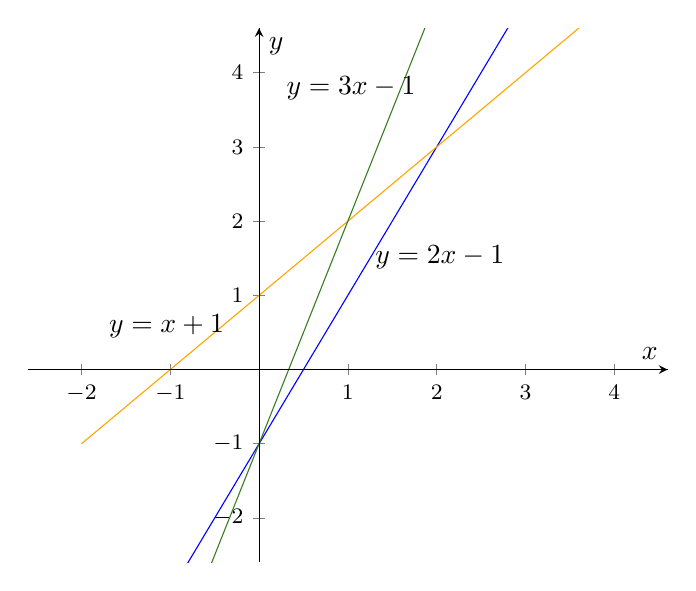
\begin{tikzpicture}
            \begin{axis}[
            width=0.8\textwidth,
            xlabel=$x$,
            ylabel=$y$,
            axis lines=middle,
            xmin=-2,
            xmax=4,
            ymin=-2,
            ymax=4,
            xtick={-2,-1,...,4},
            ytick={-2,-1,...,4},
            enlargelimits,
            ticks=both,
            %tick label style={font=\small}, % para diminuir o tamanho de fonte
            tick label style={font=\footnotesize}, % outra opção de tamanho de fonte
            % tick label style={font=\tiny} % é a menor fonte q tem
            after end axis/.code={
            \draw (axis cs:0,\pgfkeysvalueof{/pgfplots/ymin}) -- (axis cs:0,\pgfkeysvalueof{/pgfplots/ymax});
            \draw (axis cs:\pgfkeysvalueof{/pgfplots/xmin},0) -- (axis cs:\pgfkeysvalueof{/pgfplots/xmax},0);
            \node[black, above right] at (axis cs:1.2,1.22) {$y=2x-1$};
            \node[black, above right] at (axis cs:-1.8,0.3) {$y=x+1$};
            \node[black, above right] at (axis cs:0.2,3.5) {$y=3x-1$};
            }
            ]
            \addplot[domain=-2:4, blue, samples=100] {2*x-1};
            \addplot[domain=-2:4, Orange, samples=100] {x+1};
            \addplot[domain=-2:4, OliveGreen, samples=100] {3*x-1};
            \end{axis}
        \end{tikzpicture}
    \end{center}

   
        Adotando duas desigualdade, obtém-se:\\
        $
		\	\begin{cases}
				2x - 1 \; \le \; x+ 1 \;\;\; \text{(i)}\\
				x+ 1 < 3x - 1 \;\;\;\;\; \text{(ii)}
			\end{cases}
        $

        De (i), tem-se:\\
        $2x - 1 \; \le \; x+ 1 \Longrightarrow x \le 2$

        De (ii), tem-se:\\
        $x+ 1 < 3x - 1 \Longrightarrow -2x < -2 \Longrightarrow x > 1$

    Analisando os intervalos das desigualdades, tem-se:\\
    
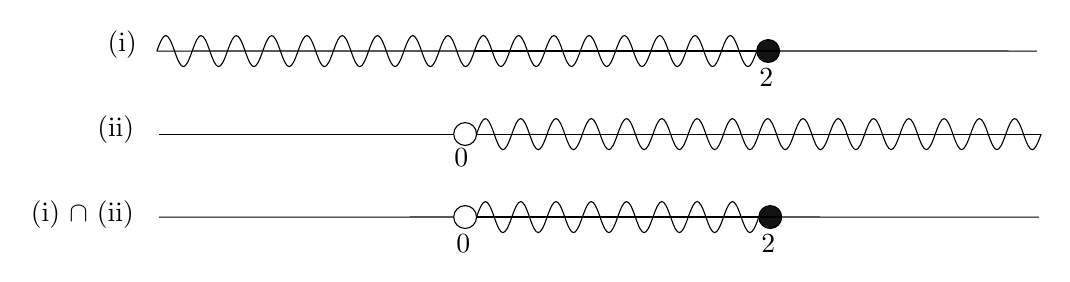
\begin{tikzpicture}[x=0.75pt,y=0.75pt,yscale=-1,xscale=1]

\draw [color={rgb, 255:red, 0; green, 0; blue, 0 }  ,draw opacity=1 ]   (101,111) -- (254,111) ;
%Straight Lines [id:da5989942174531802] 
\draw [color={rgb, 255:red, 0; green, 0; blue, 0 }  ,draw opacity=1 ]   (254,111) -- (526,111) ;
%Shape: Sine Wave Form [id:dp8605869549805791] 
\draw   (254,111) .. controls (257.46,101.08) and (259.09,101.03) .. (262.5,111) .. controls (265.91,120.97) and (267.51,121.03) .. (271,111) ;
%Shape: Sine Wave Form [id:dp8877130329379495] 
\draw   (271,111) .. controls (274.46,101.08) and (276.09,101.03) .. (279.5,111) .. controls (282.91,120.97) and (284.51,121.03) .. (288,111) ;
%Shape: Sine Wave Form [id:dp7112461966942252] 
\draw   (288,111) .. controls (291.46,101.08) and (293.09,101.03) .. (296.5,111) .. controls (299.91,120.97) and (301.51,121.03) .. (305,111) ;
%Shape: Sine Wave Form [id:dp12133983255825087] 
\draw   (305,111) .. controls (308.46,101.08) and (310.09,101.03) .. (313.5,111) .. controls (316.91,120.97) and (318.51,121.03) .. (322,111) ;
%Shape: Sine Wave Form [id:dp007731635587307384] 
\draw   (322,111) .. controls (325.46,101.08) and (327.09,101.03) .. (330.5,111) .. controls (333.91,120.97) and (335.51,121.03) .. (339,111) ;
%Shape: Sine Wave Form [id:dp4567109840020178] 
\draw   (339,111) .. controls (342.46,101.08) and (344.09,101.03) .. (347.5,111) .. controls (350.91,120.97) and (352.51,121.03) .. (356,111) ;
%Shape: Sine Wave Form [id:dp7932518413345406] 
\draw   (356,111) .. controls (359.46,101.08) and (361.09,101.03) .. (364.5,111) .. controls (367.91,120.97) and (369.51,121.03) .. (373,111) ;
%Shape: Sine Wave Form [id:dp6024246391631334] 
\draw   (373,111) .. controls (376.46,101.08) and (378.09,101.03) .. (381.5,111) .. controls (384.91,120.97) and (386.51,121.03) .. (390,111) ;
%Shape: Sine Wave Form [id:dp2041246171204938] 
\draw   (390,111) .. controls (393.46,101.08) and (395.09,101.03) .. (398.5,111) .. controls (401.91,120.97) and (403.51,121.03) .. (407,111) ;
%Shape: Sine Wave Form [id:dp9647750074548966] 
\draw   (407,111) .. controls (410.46,101.08) and (412.09,101.03) .. (415.5,111) .. controls (418.91,120.97) and (420.51,121.03) .. (424,111) ;
%Shape: Sine Wave Form [id:dp7194452227700399] 
\draw   (424,111) .. controls (427.46,101.08) and (429.09,101.03) .. (432.5,111) .. controls (435.91,120.97) and (437.51,121.03) .. (441,111) ;
%Shape: Sine Wave Form [id:dp9062116853011946] 
\draw   (441,111) .. controls (444.46,101.08) and (446.09,101.03) .. (449.5,111) .. controls (452.91,120.97) and (454.51,121.03) .. (458,111) ;
%Shape: Sine Wave Form [id:dp7886334165000064] 
\draw   (458,111) .. controls (461.46,101.08) and (463.09,101.03) .. (466.5,111) .. controls (469.91,120.97) and (471.51,121.03) .. (475,111) ;
%Shape: Sine Wave Form [id:dp894200777149057] 
\draw   (475,111) .. controls (478.46,101.08) and (480.09,101.03) .. (483.5,111) .. controls (486.91,120.97) and (488.51,121.03) .. (492,111) ;
%Shape: Sine Wave Form [id:dp5856024887828783] 
\draw   (492,111) .. controls (495.46,101.08) and (497.09,101.03) .. (500.5,111) .. controls (503.91,120.97) and (505.51,121.03) .. (509,111) ;
%Shape: Sine Wave Form [id:dp1450387631214689] 
\draw   (509,111) .. controls (512.46,101.08) and (514.09,101.03) .. (517.5,111) .. controls (520.91,120.97) and (522.51,121.03) .. (526,111) ;
%Straight Lines [id:da5776518310682439] 
\draw [color={rgb, 255:red, 0; green, 0; blue, 0 }  ,draw opacity=1 ]   (100,71) -- (253,70.97) ;
%Shape: Circle [id:dp39925187273260887] 
\draw  [fill={rgb, 255:red, 255; green, 255; blue, 255 }  ,fill opacity=1 ] (243,110.97) .. controls (243,107.93) and (245.46,105.47) .. (248.5,105.47) .. controls (251.54,105.47) and (254,107.93) .. (254,110.97) .. controls (254,114.01) and (251.54,116.47) .. (248.5,116.47) .. controls (245.46,116.47) and (243,114.01) .. (243,110.97) -- cycle ;
%Shape: Circle [id:dp6347376516422629] 
\draw  [fill={rgb, 255:red, 20; green, 19; blue, 19 }  ,fill opacity=1 ] (389,70.97) .. controls (389,67.93) and (391.46,65.47) .. (394.5,65.47) .. controls (397.54,65.47) and (400,67.93) .. (400,70.97) .. controls (400,74.01) and (397.54,76.47) .. (394.5,76.47) .. controls (391.46,76.47) and (389,74.01) .. (389,70.97) -- cycle ;
%Straight Lines [id:da6744860899053193] 
\draw [color={rgb, 255:red, 0; green, 0; blue, 0 }  ,draw opacity=1 ]   (253,70.97) -- (400,70.97) ;
%Straight Lines [id:da29054096560474596] 
\draw [color={rgb, 255:red, 0; green, 0; blue, 0 }  ,draw opacity=1 ]   (400,70.97) -- (524,71) ;
%Shape: Sine Wave Form [id:dp2745898597064571] 
\draw   (253,70.97) .. controls (256.46,61.05) and (258.09,61) .. (261.5,70.97) .. controls (264.91,80.94) and (266.51,81) .. (270,70.97) ;
%Shape: Sine Wave Form [id:dp2616841359397408] 
\draw   (270,70.97) .. controls (273.46,61.05) and (275.09,61) .. (278.5,70.97) .. controls (281.91,80.94) and (283.51,81) .. (287,70.97) ;
%Shape: Sine Wave Form [id:dp8377171544172894] 
\draw   (287,70.97) .. controls (290.46,61.05) and (292.09,61) .. (295.5,70.97) .. controls (298.91,80.94) and (300.51,81) .. (304,70.97) ;
%Shape: Sine Wave Form [id:dp6773011954115651] 
\draw   (304,70.97) .. controls (307.46,61.05) and (309.09,61) .. (312.5,70.97) .. controls (315.91,80.94) and (317.51,81) .. (321,70.97) ;
%Shape: Sine Wave Form [id:dp7632026339238038] 
\draw   (321,70.97) .. controls (324.46,61.05) and (326.09,61) .. (329.5,70.97) .. controls (332.91,80.94) and (334.51,81) .. (338,70.97) ;
%Shape: Sine Wave Form [id:dp1540572985301809] 
\draw   (338,70.97) .. controls (341.46,61.05) and (343.09,61) .. (346.5,70.97) .. controls (349.91,80.94) and (351.51,81) .. (355,70.97) ;
%Shape: Sine Wave Form [id:dp395101011360274] 
\draw   (355,70.97) .. controls (358.46,61.05) and (360.09,61) .. (363.5,70.97) .. controls (366.91,80.94) and (368.51,81) .. (372,70.97) ;
%Shape: Sine Wave Form [id:dp15731756857858015] 
\draw   (372,70.97) .. controls (375.46,61.05) and (377.09,61) .. (380.5,70.97) .. controls (383.91,80.94) and (385.51,81) .. (389,70.97) ;
%Straight Lines [id:da25941572796049117] 
\draw [color={rgb, 255:red, 0; green, 0; blue, 0 }  ,draw opacity=1 ]   (101,151) -- (243,150.97) ;
%Shape: Circle [id:dp9212476290673159] 
\draw  [fill={rgb, 255:red, 255; green, 255; blue, 255 }  ,fill opacity=1 ] (243,150.97) .. controls (243,147.93) and (245.46,145.47) .. (248.5,145.47) .. controls (251.54,145.47) and (254,147.93) .. (254,150.97) .. controls (254,154.01) and (251.54,156.47) .. (248.5,156.47) .. controls (245.46,156.47) and (243,154.01) .. (243,150.97) -- cycle ;
%Shape: Circle [id:dp22223646257016583] 
\draw  [fill={rgb, 255:red, 20; green, 19; blue, 19 }  ,fill opacity=1 ] (390,150.97) .. controls (390,147.93) and (392.46,145.47) .. (395.5,145.47) .. controls (398.54,145.47) and (401,147.93) .. (401,150.97) .. controls (401,154.01) and (398.54,156.47) .. (395.5,156.47) .. controls (392.46,156.47) and (390,154.01) .. (390,150.97) -- cycle ;
%Straight Lines [id:da38976820602908635] 
\draw [color={rgb, 255:red, 0; green, 0; blue, 0 }  ,draw opacity=1 ]   (254,150.97) -- (401,150.97) ;
%Straight Lines [id:da7071107542846851] 
\draw [color={rgb, 255:red, 0; green, 0; blue, 0 }  ,draw opacity=1 ]   (401,150.97) -- (525,151) ;
%Shape: Sine Wave Form [id:dp6145867461292012] 
\draw   (254,150.97) .. controls (257.46,141.05) and (259.09,141) .. (262.5,150.97) .. controls (265.91,160.94) and (267.51,161) .. (271,150.97) ;
%Shape: Sine Wave Form [id:dp34156769473399407] 
\draw   (271,150.97) .. controls (274.46,141.05) and (276.09,141) .. (279.5,150.97) .. controls (282.91,160.94) and (284.51,161) .. (288,150.97) ;
%Shape: Sine Wave Form [id:dp4836316937186782] 
\draw   (288,150.97) .. controls (291.46,141.05) and (293.09,141) .. (296.5,150.97) .. controls (299.91,160.94) and (301.51,161) .. (305,150.97) ;
%Shape: Sine Wave Form [id:dp10002842039980697] 
\draw   (305,150.97) .. controls (308.46,141.05) and (310.09,141) .. (313.5,150.97) .. controls (316.91,160.94) and (318.51,161) .. (322,150.97) ;
%Shape: Sine Wave Form [id:dp4535657271206619] 
\draw   (322,150.97) .. controls (325.46,141.05) and (327.09,141) .. (330.5,150.97) .. controls (333.91,160.94) and (335.51,161) .. (339,150.97) ;
%Shape: Sine Wave Form [id:dp8642601597958188] 
\draw   (339,150.97) .. controls (342.46,141.05) and (344.09,141) .. (347.5,150.97) .. controls (350.91,160.94) and (352.51,161) .. (356,150.97) ;
%Shape: Sine Wave Form [id:dp30455456891621746] 
\draw   (356,150.97) .. controls (359.46,141.05) and (361.09,141) .. (364.5,150.97) .. controls (367.91,160.94) and (369.51,161) .. (373,150.97) ;
%Shape: Sine Wave Form [id:dp5334802978414701] 
\draw   (373,150.97) .. controls (376.46,141.05) and (378.09,141) .. (381.5,150.97) .. controls (384.91,160.94) and (386.51,161) .. (390,150.97) ;
%Shape: Sine Wave Form [id:dp26426672807314056] 
\draw   (117,71) .. controls (120.46,61.08) and (122.09,61.03) .. (125.5,71) .. controls (128.91,80.97) and (130.51,81.03) .. (134,71) ;
%Shape: Sine Wave Form [id:dp06911201357868024] 
\draw   (134,71) .. controls (137.46,61.08) and (139.09,61.03) .. (142.5,71) .. controls (145.91,80.97) and (147.51,81.03) .. (151,71) ;
%Shape: Sine Wave Form [id:dp7018300153952175] 
\draw   (151,71) .. controls (154.46,61.08) and (156.09,61.03) .. (159.5,71) .. controls (162.91,80.97) and (164.51,81.03) .. (168,71) ;
%Shape: Sine Wave Form [id:dp6264184723965356] 
\draw   (168,71) .. controls (171.46,61.08) and (173.09,61.03) .. (176.5,71) .. controls (179.91,80.97) and (181.51,81.03) .. (185,71) ;
%Shape: Sine Wave Form [id:dp06421947643580994] 
\draw   (185,71) .. controls (188.46,61.08) and (190.09,61.03) .. (193.5,71) .. controls (196.91,80.97) and (198.51,81.03) .. (202,71) ;
%Shape: Sine Wave Form [id:dp4026217270841934] 
\draw   (202,71) .. controls (205.46,61.08) and (207.09,61.03) .. (210.5,71) .. controls (213.91,80.97) and (215.51,81.03) .. (219,71) ;
%Shape: Sine Wave Form [id:dp8985326967167646] 
\draw   (219,71) .. controls (222.46,61.08) and (224.09,61.03) .. (227.5,71) .. controls (230.91,80.97) and (232.51,81.03) .. (236,71) ;
%Shape: Sine Wave Form [id:dp8786417702119775] 
\draw   (236,71) .. controls (239.46,61.08) and (241.09,61.03) .. (244.5,71) .. controls (247.91,80.97) and (249.51,81.03) .. (253,71) ;
%Shape: Sine Wave Form [id:dp9223032032770362] 
\draw   (100,71) .. controls (103.46,61.08) and (105.09,61.03) .. (108.5,71) .. controls (111.91,80.97) and (113.51,81.03) .. (117,71) ;

\draw (75,60) node [anchor=north west][inner sep=0.75pt]   [align=left] {(i)};
% Text Node
\draw (38,142) node [anchor=north west][inner sep=0.75pt]   [align=left] {(i) $\cap$ (ii)};
% Text Node
\draw (70,101) node [anchor=north west][inner sep=0.75pt]   [align=left] {(ii)};
% Text Node
\draw (242,117) node [anchor=north west][inner sep=0.75pt]   [align=left] {0};
% Text Node
\draw (389,78) node [anchor=north west][inner sep=0.75pt]   [align=left] {2};
% Text Node
\draw (243,158) node [anchor=north west][inner sep=0.75pt]   [align=left] {0};
% Text Node
\draw (390,158) node [anchor=north west][inner sep=0.75pt]   [align=left] {2};
\end{tikzpicture}

        Logo, $S = (1, 2] \text{ ou } S = \{  x \in \mathbb{R} \mid x \le 2\}$.\\
        
        
			%%%%%%%%%%%%%%%%%%%%%%%%%%%%%%%%%%%%%%%%%%
			\item 
			$
			\ fx=\begin{cases}
				3x-1 > 5x+2 \\
				4x+3 < 7x-11
			\end{cases}
			$ \;\;(Sistema de inequações)\\

        Resolução: \\
        Considera-se $x \in \mathbb{R}$.\\
        Primeiro, nomeia-se as desigualdades:

        $
			\ fx=\begin{cases}
				3x-1 > 5x+2 \;\;\; \text{(i)} \\
				4x+3 < 7x-11\;\;\; \text{(ii)}
			\end{cases}
			$ 

        De (i) tem-se:\\
            $3x-1 > 5x+2 \Longrightarrow -2x >3 \Longrightarrow x < -\dfrac{3}{2}$
            
        De (ii) tem-se:\\
            $4x+3 < 7x-11 \Longrightarrow -3x<-14 
            \Longrightarrow x > \dfrac{14}{3}$
            
        Analisando os intervalos das desigualdades, tem-se\\
        
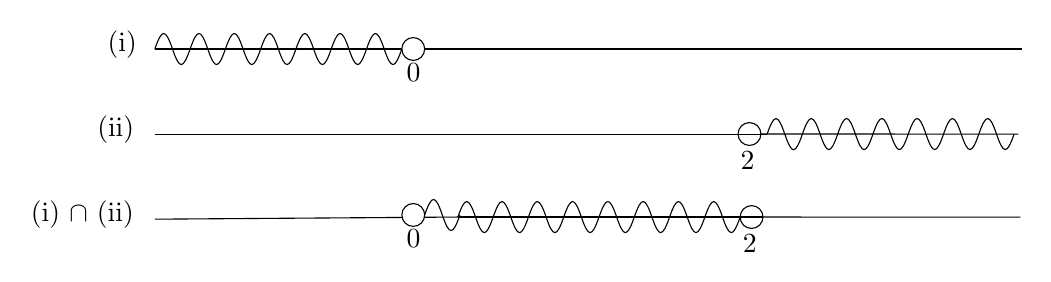
\begin{tikzpicture}[x=0.75pt,y=0.75pt,yscale=-1,xscale=1]
\draw [color={rgb, 255:red, 0; green, 0; blue, 0 }  ,draw opacity=1 ]   (108,70) -- (254,70) ;
%Straight Lines [id:da5989942174531802] 
\draw [color={rgb, 255:red, 0; green, 0; blue, 0 }  ,draw opacity=1 ]   (254,70) -- (526,70) ;
%Straight Lines [id:da5776518310682439] 
\draw [color={rgb, 255:red, 0; green, 0; blue, 0 }  ,draw opacity=1 ]   (108,111) -- (256,111) ;
%Shape: Circle [id:dp39925187273260887] 
\draw  [fill={rgb, 255:red, 255; green, 255; blue, 255 }  ,fill opacity=1 ] (227,70) .. controls (227,66.96) and (229.46,64.5) .. (232.5,64.5) .. controls (235.54,64.5) and (238,66.96) .. (238,70) .. controls (238,73.04) and (235.54,75.5) .. (232.5,75.5) .. controls (229.46,75.5) and (227,73.04) .. (227,70) -- cycle ;
%Shape: Circle [id:dp6347376516422629] 
\draw  [fill={rgb, 255:red, 255; green, 255; blue, 255 }  ,fill opacity=1 ] (389,110.97) .. controls (389,107.93) and (391.46,105.47) .. (394.5,105.47) .. controls (397.54,105.47) and (400,107.93) .. (400,110.97) .. controls (400,114.01) and (397.54,116.47) .. (394.5,116.47) .. controls (391.46,116.47) and (389,114.01) .. (389,110.97) -- cycle ;
%Straight Lines [id:da6744860899053193] 
\draw [color={rgb, 255:red, 0; green, 0; blue, 0 }  ,draw opacity=1 ]   (256,111) -- (403,111) ;
%Straight Lines [id:da29054096560474596] 
\draw [color={rgb, 255:red, 0; green, 0; blue, 0 }  ,draw opacity=1 ]   (400,110.97) -- (524,111) ;
%Shape: Sine Wave Form [id:dp2745898597064571] 
\draw   (420,110.97) .. controls (423.46,101.05) and (425.09,101) .. (428.5,110.97) .. controls (431.91,120.94) and (433.51,121) .. (437,110.97) ;
%Shape: Sine Wave Form [id:dp2616841359397408] 
\draw   (437,110.97) .. controls (440.46,101.05) and (442.09,101) .. (445.5,110.97) .. controls (448.91,120.94) and (450.51,121) .. (454,110.97) ;
%Shape: Sine Wave Form [id:dp8377171544172894] 
\draw   (454,110.97) .. controls (457.46,101.05) and (459.09,101) .. (462.5,110.97) .. controls (465.91,120.94) and (467.51,121) .. (471,110.97) ;
%Shape: Sine Wave Form [id:dp6773011954115651] 
\draw   (471,110.97) .. controls (474.46,101.05) and (476.09,101) .. (479.5,110.97) .. controls (482.91,120.94) and (484.51,121) .. (488,110.97) ;
%Shape: Sine Wave Form [id:dp7632026339238038] 
\draw   (488,110.97) .. controls (491.46,101.05) and (493.09,101) .. (496.5,110.97) .. controls (499.91,120.94) and (501.51,121) .. (505,110.97) ;
%Shape: Sine Wave Form [id:dp1540572985301809] 
\draw   (505,110.97) .. controls (508.46,101.05) and (510.09,101) .. (513.5,110.97) .. controls (516.91,120.94) and (518.51,121) .. (522,110.97) ;
%Straight Lines [id:da25941572796049117] 
\draw [color={rgb, 255:red, 0; green, 0; blue, 0 }  ,draw opacity=1 ]   (108,152) -- (254,150.97) ;
%Shape: Circle [id:dp9212476290673159] 
\draw  [fill={rgb, 255:red, 255; green, 255; blue, 255 }  ,fill opacity=1 ] (227,149.97) .. controls (227,146.93) and (229.46,144.47) .. (232.5,144.47) .. controls (235.54,144.47) and (238,146.93) .. (238,149.97) .. controls (238,153.01) and (235.54,155.47) .. (232.5,155.47) .. controls (229.46,155.47) and (227,153.01) .. (227,149.97) -- cycle ;
%Shape: Circle [id:dp22223646257016583] 
\draw  [fill={rgb, 255:red, 255; green, 255; blue, 255 }  ,fill opacity=1 ] (390,150.97) .. controls (390,147.93) and (392.46,145.47) .. (395.5,145.47) .. controls (398.54,145.47) and (401,147.93) .. (401,150.97) .. controls (401,154.01) and (398.54,156.47) .. (395.5,156.47) .. controls (392.46,156.47) and (390,154.01) .. (390,150.97) -- cycle ;
%Straight Lines [id:da38976820602908635] 
\draw [color={rgb, 255:red, 0; green, 0; blue, 0 }  ,draw opacity=1 ]   (254,150.97) -- (401,150.97) ;
%Straight Lines [id:da7071107542846851] 
\draw [color={rgb, 255:red, 0; green, 0; blue, 0 }  ,draw opacity=1 ]   (401,150.97) -- (525,151) ;
%Shape: Sine Wave Form [id:dp6145867461292012] 
\draw   (254,150.97) .. controls (257.46,141.05) and (259.09,141) .. (262.5,150.97) .. controls (265.91,160.94) and (267.51,161) .. (271,150.97) ;
%Shape: Sine Wave Form [id:dp34156769473399407] 
\draw   (271,150.97) .. controls (274.46,141.05) and (276.09,141) .. (279.5,150.97) .. controls (282.91,160.94) and (284.51,161) .. (288,150.97) ;
%Shape: Sine Wave Form [id:dp4836316937186782] 
\draw   (288,150.97) .. controls (291.46,141.05) and (293.09,141) .. (296.5,150.97) .. controls (299.91,160.94) and (301.51,161) .. (305,150.97) ;
%Shape: Sine Wave Form [id:dp10002842039980697] 
\draw   (305,150.97) .. controls (308.46,141.05) and (310.09,141) .. (313.5,150.97) .. controls (316.91,160.94) and (318.51,161) .. (322,150.97) ;
%Shape: Sine Wave Form [id:dp4535657271206619] 
\draw   (322,150.97) .. controls (325.46,141.05) and (327.09,141) .. (330.5,150.97) .. controls (333.91,160.94) and (335.51,161) .. (339,150.97) ;
%Shape: Sine Wave Form [id:dp8642601597958188] 
\draw   (339,150.97) .. controls (342.46,141.05) and (344.09,141) .. (347.5,150.97) .. controls (350.91,160.94) and (352.51,161) .. (356,150.97) ;
%Shape: Sine Wave Form [id:dp30455456891621746] 
\draw   (356,150.97) .. controls (359.46,141.05) and (361.09,141) .. (364.5,150.97) .. controls (367.91,160.94) and (369.51,161) .. (373,150.97) ;
%Shape: Sine Wave Form [id:dp5334802978414701] 
\draw   (373,150.97) .. controls (376.46,141.05) and (378.09,141) .. (381.5,150.97) .. controls (384.91,160.94) and (386.51,161) .. (390,150.97) ;
%Shape: Sine Wave Form [id:dp26426672807314056] 
\draw   (125,70) .. controls (128.46,60.08) and (130.09,60.03) .. (133.5,70) .. controls (136.91,79.97) and (138.51,80.03) .. (142,70) ;
%Shape: Sine Wave Form [id:dp06911201357868024] 
\draw   (142,70) .. controls (145.46,60.08) and (147.09,60.03) .. (150.5,70) .. controls (153.91,79.97) and (155.51,80.03) .. (159,70) ;
%Shape: Sine Wave Form [id:dp7018300153952175] 
\draw   (159,70) .. controls (162.46,60.08) and (164.09,60.03) .. (167.5,70) .. controls (170.91,79.97) and (172.51,80.03) .. (176,70) ;
%Shape: Sine Wave Form [id:dp6264184723965356] 
\draw   (176,70) .. controls (179.46,60.08) and (181.09,60.03) .. (184.5,70) .. controls (187.91,79.97) and (189.51,80.03) .. (193,70) ;
%Shape: Sine Wave Form [id:dp06421947643580994] 
\draw   (193,70) .. controls (196.46,60.08) and (198.09,60.03) .. (201.5,70) .. controls (204.91,79.97) and (206.51,80.03) .. (210,70) ;
%Shape: Sine Wave Form [id:dp4026217270841934] 
\draw   (210,70) .. controls (213.46,60.08) and (215.09,60.03) .. (218.5,70) .. controls (221.91,79.97) and (223.51,80.03) .. (227,70) ;
%Shape: Sine Wave Form [id:dp8786417702119775] 
\draw   (403,111) .. controls (406.46,101.08) and (408.09,101.03) .. (411.5,111) .. controls (414.91,120.97) and (416.51,121.03) .. (420,111) ;
%Shape: Sine Wave Form [id:dp9223032032770362] 
\draw   (108,70) .. controls (111.46,60.08) and (113.09,60.03) .. (116.5,70) .. controls (119.91,79.97) and (121.51,80.03) .. (125,70) ;
%Shape: Sine Wave Form [id:dp9387697145183471] 
\draw   (238,149.97) .. controls (241.46,140.05) and (243.09,140) .. (246.5,149.97) .. controls (249.91,159.94) and (251.51,160) .. (255,149.97) ;

% Text Node
\draw (84,60) node [anchor=north west][inner sep=0.75pt]   [align=left] {(i)};
% Text Node
\draw (47,142) node [anchor=north west][inner sep=0.75pt]   [align=left] {(i) $\cap$ (ii)};
% Text Node
\draw (79,101) node [anchor=north west][inner sep=0.75pt]   [align=left] {(ii)};
% Text Node
\draw (228,76) node [anchor=north west][inner sep=0.75pt]   [align=left] {0};
% Text Node
\draw (389,118) node [anchor=north west][inner sep=0.75pt]   [align=left] {2};
% Text Node
\draw (228,156) node [anchor=north west][inner sep=0.75pt]   [align=left] {0};
% Text Node
\draw (390,158) node [anchor=north west][inner sep=0.75pt]   [align=left] {2};
\end{tikzpicture}

   Deste modo, como (i) $\cap$ (ii) = \slashzero, o sistema não tem solução.
   
			%%%%%%%%%%%%%%%%%%%%%%%%%%%%%%%%%%%%%%%%%%
			\item $(2x+5)(-3x+7) < 0$ \;\; (Inequação produto)\\
   
    Em primeiro lugar, faz-se um estudo do sinal de cada termo. Sendo o primeiro termo (i) igual a $2x+5$ e o segundo termo (ii) igual a $(-3x+7)$.\\
    
    A análise de (i):\\
    \[
    2x+5 = 0 \Longrightarrow 2x = -5 \Longrightarrow x = -\dfrac{5}{2}
    \]
    \[
    2x+5 < 0 \Longrightarrow 2x < -5 \Longrightarrow x < -\dfrac{5}{2}
    \]
    \[
    2x+5 > 0 \Longrightarrow 2x > -5 \Longrightarrow x > -\dfrac{5}{2}
    \]
    Na reta real tem-se:
    \begin{center}
            \begin{tikzpicture}[x=0.75pt,y=0.75pt,yscale=-1,xscale=1]
                \draw [color={rgb, 255:red, 243; green, 43; blue, 11 }  ,draw opacity=1 ]   (90,90) -- (240,90) ;
                \draw [color={rgb, 255:red, 74; green, 144; blue, 226 }  ,draw opacity=1 ]   (240,90) -- (391,90) ;
                \draw    (240,85) -- (240,94) ;
                \draw    (321,13.75) -- (163,159.75) ;
                \draw (231,95) node [anchor=north west][inner sep=0.75pt]   [align=left] {$-\dfrac{5}{2}$};
                \draw (258,71) node [anchor=north west][inner sep=0.75pt]   [align=left] {$+$ \ \ \ \ $+$ \ \ \ \ $+$ \ \ \ \ $+$};
                \draw (94,96) node [anchor=north west][inner sep=0.75pt]   [align=left] {$-$ \ \ \ $-$ \ \ \ $-$ \ \ \ $-$};
            \end{tikzpicture}                  
    \end{center}

    A análise de (ii):\\
            \[
            -3x+7=0 \Longrightarrow 3x=7 \Longrightarrow x= \dfrac{7}{3}
            \]
            \[
            -3x+7<0 \Longrightarrow 3x<7 \Longrightarrow x< \dfrac{7}{3}
            \]
            \[
            -3x+7>0 \Longrightarrow 3x>7 \Longrightarrow x> \dfrac{7}{3}
            \]
    Na reta real tem-se:

    Assim, 

            
\begin{center}
\begin{tikzpicture}[x=0.75pt,y=0.75pt,yscale=-1,xscale=1]

\draw [color={rgb, 255:red, 74; green, 144; blue, 226 }  ,draw opacity=1 ]   (90,90) -- (240,90) ;
%Straight Lines [id:da9966835219779178] 
\draw [color={rgb, 255:red, 243; green, 11; blue, 39 }  ,draw opacity=1 ]   (240,90) -- (391,90) ;
%Straight Lines [id:da10431794756153057] 
\draw    (240,85) -- (240,94) ;
%Straight Lines [id:da260308124484147] 
\draw    (161,15) -- (313,159) ;

\draw (224,100) node [anchor=north west][inner sep=0.75pt]   [align=left] {$\dfrac{7}{3}$};
% Text Node
\draw (92,71) node [anchor=north west][inner sep=0.75pt]   [align=left] {$+$ \ \ \ \ $+$ \ \ \ \ $+$ \ \ \ \ $+$};
% Text Node
\draw (270,94) node [anchor=north west][inner sep=0.75pt]   [align=left] {$-$ \ \ \ $-$ \ \ \ $-$ \ \ \ $-$};
\end{tikzpicture}
\end{center}

        Analisando os dois termos juntos tem-se

\begin{tikzpicture}[x=0.75pt,y=0.75pt,yscale=-1,xscale=1]

\draw [color={rgb, 255:red, 74; green, 144; blue, 226 }  ,draw opacity=1 ]   (101,126) -- (338,125) ;
%Shape: Circle [id:dp17867708220140965] 
\draw  [fill={rgb, 255:red, 255; green, 255; blue, 255 }  ,fill opacity=1 ] (338,125) .. controls (338,121.96) and (340.46,119.5) .. (343.5,119.5) .. controls (346.54,119.5) and (349,121.96) .. (349,125) .. controls (349,128.04) and (346.54,130.5) .. (343.5,130.5) .. controls (340.46,130.5) and (338,128.04) .. (338,125) -- cycle ;
%Straight Lines [id:da32527376127659346] 
\draw [color={rgb, 255:red, 247; green, 45; blue, 30 }  ,draw opacity=1 ]   (349,125) -- (527,126) ;
%Straight Lines [id:da9329789261744439] 
\draw [color={rgb, 255:red, 243; green, 43; blue, 11 }  ,draw opacity=1 ]   (102,69) -- (213,70) ;
%Shape: Circle [id:dp25271154714791644] 
\draw  [fill={rgb, 255:red, 255; green, 255; blue, 255 }  ,fill opacity=1 ] (213,70) .. controls (213,66.96) and (215.46,64.5) .. (218.5,64.5) .. controls (221.54,64.5) and (224,66.96) .. (224,70) .. controls (224,73.04) and (221.54,75.5) .. (218.5,75.5) .. controls (215.46,75.5) and (213,73.04) .. (213,70) -- cycle ;
%Straight Lines [id:da9967480313894097] 
\draw [color={rgb, 255:red, 74; green, 144; blue, 226 }  ,draw opacity=1 ]   (224,70) -- (452,70) ;
%Straight Lines [id:da9645451066891781] 
\draw [color={rgb, 255:red, 74; green, 144; blue, 226 }  ,draw opacity=1 ]   (452,70) -- (525,70) ;
%Straight Lines [id:da9568143770136996] 
\draw [color={rgb, 255:red, 74; green, 144; blue, 226 }  ,draw opacity=1 ]   (224,187) -- (339,187) ;
%Shape: Circle [id:dp8487660824468224] 
\draw  [fill={rgb, 255:red, 255; green, 255; blue, 255 }  ,fill opacity=1 ] (339,187) .. controls (339,183.96) and (341.46,181.5) .. (344.5,181.5) .. controls (347.54,181.5) and (350,183.96) .. (350,187) .. controls (350,190.04) and (347.54,192.5) .. (344.5,192.5) .. controls (341.46,192.5) and (339,190.04) .. (339,187) -- cycle ;
%Straight Lines [id:da24916310298444788] 
\draw [color={rgb, 255:red, 247; green, 7; blue, 34 }  ,draw opacity=1 ]   (350,187) -- (453,188) ;
%Straight Lines [id:da23935991401671264] 
\draw [color={rgb, 255:red, 192; green, 14; blue, 8 }  ,draw opacity=1 ]   (453,188) -- (526,188) ;
%Shape: Circle [id:dp7910642357859696] 
\draw  [fill={rgb, 255:red, 255; green, 255; blue, 255 }  ,fill opacity=1 ] (213,187) .. controls (213,183.96) and (215.46,181.5) .. (218.5,181.5) .. controls (221.54,181.5) and (224,183.96) .. (224,187) .. controls (224,190.04) and (221.54,192.5) .. (218.5,192.5) .. controls (215.46,192.5) and (213,190.04) .. (213,187) -- cycle ;
%Straight Lines [id:da6017888128884432] 
\draw [color={rgb, 255:red, 235; green, 11; blue, 11 }  ,draw opacity=1 ]   (105,188) -- (213,187) ;

% Text Node
\draw (75,60) node [anchor=north west][inner sep=0.75pt]   [align=left] {(i)};
% Text Node
\draw (75,118) node [anchor=north west][inner sep=0.75pt]   [align=left] {(ii)};
% Text Node
\draw (38,178) node [anchor=north west][inner sep=0.75pt]   [align=left] {Produto};
% Text Node
\draw (206,194) node [anchor=north west][inner sep=0.75pt]   [align=left] {$-\dfrac{5}{2}$};
% Text Node
\draw (340.5,195) node [anchor=north west][inner sep=0.75pt]   [align=left] {$\dfrac{7}{3}$};
% Text Node
\draw (206,76) node [anchor=north west][inner sep=0.75pt]   [align=left] {$-\dfrac{5}{2}$};
% Text Node
\draw (257,49) node [anchor=north west][inner sep=0.75pt]   [align=left] {$+$ \ \ \ \ \ \ \ \ $+$ \ \ \ \ \ \ \ \ \ $+$ \ \ \ \ \ \ \ \ \ $+$ \ \ \ \ \ \ \ \ \ $+$};
% Text Node
\draw (108,106) node [anchor=north west][inner sep=0.75pt]   [align=left] {$+$ \ \ \ \ \ \ \ \ $+$ \ \ \ \ \ \ \ \ \ $+$ \ \ \ \ \ \ \ \ \ $+$};
% Text Node
\draw (244,166) node [anchor=north west][inner sep=0.75pt]   [align=left] { $+$ \ \ \ \ \ \ \ \ \ $+$};
% Text Node
\draw (116,169) node [anchor=north west][inner sep=0.75pt]   [align=left] {$-$ \ \ \ \ $-$ \ \ \ \ $-$};
% Text Node
\draw (376,168) node [anchor=north west][inner sep=0.75pt]   [align=left] {$-$ \ \ \ \ $-$ \ \ \ \ $-$ \ \ \ \ $-$};
% Text Node
\draw (112,47) node [anchor=north west][inner sep=0.75pt]   [align=left] {$-$ \ \ \ \ $-$ \ \ \ \ $-$};
% Text Node
\draw (356,107) node [anchor=north west][inner sep=0.75pt]   [align=left] { $-$ \ \ \ \ $-$ \ \ \ \ $-$ \ \ \ \ $-$};
% Text Node
\draw (340.5,133) node [anchor=north west][inner sep=0.75pt]   [align=left] {$\dfrac{7}{3}$};
\end{tikzpicture}

        A solução está no intervalo em que o produto é menor do que zero.\\
        
        S = $\left(- \infty, -\dfrac{5}{2} \right) U \left( \dfrac{7}{3}, + \infty \right)$ ou S = $\{ x \in \mathbb{R} \mid x< - \dfrac{5}{2} \text{ ou } \dfrac{7}{3} \}$
        
			%%%%%%%%%%%%%%%%%%%%%%%%%%%%%%%%%%%%%%%%%%
			\item $ \dfrac{-4x-6}{5x-10} \ge 0$ \;\; (Inequação quociente)\\
   
    É necessário verificar a condição de existência da  inequação.\\
    \[
    5x-10 \neq 0 \Longrightarrow 5x \neq 10 \Longrightarrow x \neq 2
    \]
    
    Em seguida, faz-se um estudo do sinal de cada termo. Sendo o primeiro termo (i) igual a $-4x-6$ e o segundo termo (ii) igual a $5x-10$.\\
    
    A análise de (i):\\
    
    \[
    -4x-6 = 0 \Longrightarrow -4x = 6 \Longrightarrow x = -\dfrac{6}{4} \Longrightarrow x = -\dfrac{3}{2}
    \]
    \[
    -4x-6 < 0 \Longrightarrow -4x < 6 \Longrightarrow x > -\dfrac{6}{4} \Longrightarrow x > -\dfrac{3}{2}
    \]
    \[
    -4x-6 > 0 \Longrightarrow -4x > 6 \Longrightarrow x < -\dfrac{6}{4} \Longrightarrow x < -\dfrac{3}{2}
    \]
    
    Na reta real tem-se:\\
    
    \begin{center}
\begin{tikzpicture}[x=0.75pt,y=0.75pt,yscale=-1,xscale=1]

\draw [color={rgb, 255:red, 74; green, 144; blue, 226 }  ,draw opacity=1 ]   (90,90) -- (240,90) ;
%Straight Lines [id:da9966835219779178] 
\draw [color={rgb, 255:red, 243; green, 11; blue, 39 }  ,draw opacity=1 ]   (240,90) -- (391,90) ;
%Straight Lines [id:da10431794756153057] 
\draw    (240,85) -- (240,94) ;
%Straight Lines [id:da260308124484147] 
\draw    (161,15) -- (313,159) ;

\draw (224,100) node [anchor=north west][inner sep=0.75pt]   [align=left] {$-\dfrac{3}{2}$};
% Text Node
\draw (92,71) node [anchor=north west][inner sep=0.75pt]   [align=left] {$+$ \ \ \ \ $+$ \ \ \ \ $+$ \ \ \ \ $+$};
% Text Node
\draw (270,94) node [anchor=north west][inner sep=0.75pt]   [align=left] {$-$ \ \ \ $-$ \ \ \ $-$ \ \ \ $-$};
\end{tikzpicture}
\end{center}

     A análise de (ii):\\
     \[
     5x-10 < 0 \Longrightarrow 5x < 10 \Longrightarrow x < 2
     \]
     \[
     5x-10 > 0 \Longrightarrow 5x > 10 \Longrightarrow x > 2
     \]

    \begin{center}
            \begin{tikzpicture}[x=0.75pt,y=0.75pt,yscale=-1,xscale=1]
                \draw [color={rgb, 255:red, 243; green, 43; blue, 11 }  ,draw opacity=1 ]   (90,90) -- (240,90) ;
                \draw [color={rgb, 255:red, 74; green, 144; blue, 226 }  ,draw opacity=1 ]   (240,90) -- (391,90) ;
                \draw    (240,85) -- (240,94) ;
                \draw    (321,13.75) -- (163,159.75) ;
                \draw (231,95) node [anchor=north west][inner sep=0.75pt]   [align=left] {$2$};
                \draw (258,71) node [anchor=north west][inner sep=0.75pt]   [align=left] {$+$ \ \ \ \ $+$ \ \ \ \ $+$ \ \ \ \ $+$};
                \draw (94,96) node [anchor=north west][inner sep=0.75pt]   [align=left] {$-$ \ \ \ $-$ \ \ \ $-$ \ \ \ $-$};
            \end{tikzpicture}                  
    \end{center}

   Analisando os dois termos juntos tem-se\\

\begin{tikzpicture}[x=0.75pt,y=0.75pt,yscale=-1,xscale=1]

%Straight Lines [id:da52716338522685] 
\draw [color={rgb, 255:red, 226; green, 79; blue, 74 }  ,draw opacity=1 ]   (101,126) -- (338,125) ;
%Shape: Circle [id:dp17867708220140965] 
\draw  [fill={rgb, 255:red, 255; green, 255; blue, 255 }  ,fill opacity=1 ] (338,125) .. controls (338,121.96) and (340.46,119.5) .. (343.5,119.5) .. controls (346.54,119.5) and (349,121.96) .. (349,125) .. controls (349,128.04) and (346.54,130.5) .. (343.5,130.5) .. controls (340.46,130.5) and (338,128.04) .. (338,125) -- cycle ;
%Straight Lines [id:da32527376127659346] 
\draw [color={rgb, 255:red, 74; green, 144; blue, 226 }  ,draw opacity=1 ]   (349,125) -- (527,126) ;
%Straight Lines [id:da9329789261744439] 
\draw [color={rgb, 255:red, 74; green, 144; blue, 226 }  ,draw opacity=1 ]   (102,69) -- (213,70) ;
%Shape: Circle [id:dp25271154714791644] 
\draw  [fill={rgb, 255:red, 0; green, 0; blue, 0 }  ,fill opacity=1 ] (213,70) .. controls (213,66.96) and (215.46,64.5) .. (218.5,64.5) .. controls (221.54,64.5) and (224,66.96) .. (224,70) .. controls (224,73.04) and (221.54,75.5) .. (218.5,75.5) .. controls (215.46,75.5) and (213,73.04) .. (213,70) -- cycle ;
%Straight Lines [id:da9967480313894097] 
\draw [color={rgb, 255:red, 226; green, 85; blue, 74 }  ,draw opacity=1 ]   (224,70) -- (452,70) ;
%Straight Lines [id:da9645451066891781] 
\draw [color={rgb, 255:red, 226; green, 95; blue, 74 }  ,draw opacity=1 ]   (452,70) -- (525,70) ;
%Straight Lines [id:da9568143770136996] 
\draw [color={rgb, 255:red, 74; green, 144; blue, 226 }  ,draw opacity=1 ]   (224,187) -- (339,187) ;
%Shape: Circle [id:dp8487660824468224] 
\draw  [fill={rgb, 255:red, 255; green, 255; blue, 255 }  ,fill opacity=1 ] (339,187) .. controls (339,183.96) and (341.46,181.5) .. (344.5,181.5) .. controls (347.54,181.5) and (350,183.96) .. (350,187) .. controls (350,190.04) and (347.54,192.5) .. (344.5,192.5) .. controls (341.46,192.5) and (339,190.04) .. (339,187) -- cycle ;
%Straight Lines [id:da24916310298444788] 
\draw [color={rgb, 255:red, 240; green, 35; blue, 60 }  ,draw opacity=1 ]   (350,187) -- (453,188) ;
%Straight Lines [id:da23935991401671264] 
\draw [color={rgb, 255:red, 240; green, 35; blue, 60 }  ,draw opacity=1 ]   (453,188) -- (526,188) ;
%Shape: Circle [id:dp7910642357859696] 
\draw  [fill={rgb, 255:red, 0; green, 0; blue, 0 }  ,fill opacity=1 ] (213,187) .. controls (213,183.96) and (215.46,181.5) .. (218.5,181.5) .. controls (221.54,181.5) and (224,183.96) .. (224,187) .. controls (224,190.04) and (221.54,192.5) .. (218.5,192.5) .. controls (215.46,192.5) and (213,190.04) .. (213,187) -- cycle ;
%Straight Lines [id:da6017888128884432] 
\draw [color={rgb, 255:red, 226; green, 90; blue, 74 }  ,draw opacity=1 ]   (105,188) -- (213,187) ;


% Text Node
\draw (75,60) node [anchor=north west][inner sep=0.75pt]   [align=left] {(i)};
% Text Node
\draw (75,118) node [anchor=north west][inner sep=0.75pt]   [align=left] {(ii)};
% Text Node
\draw (26,178) node [anchor=north west][inner sep=0.75pt]   [align=left] {Quociente};
% Text Node
\draw (214,194) node [anchor=north west][inner sep=0.75pt]   [align=left] {$-\dfrac{3}{2}$};
% Text Node
\draw (340.5,196) node [anchor=north west][inner sep=0.75pt]   [align=left] {2};
% Text Node
\draw (213,76) node [anchor=north west][inner sep=0.75pt]   [align=left] {$-\dfrac{3}{2}$};
% Text Node
\draw (108,48) node [anchor=north west][inner sep=0.75pt]   [align=left] {$+$ \ \ \ \ \ \ \ \ \ $+$};
% Text Node
\draw (355,106) node [anchor=north west][inner sep=0.75pt]   [align=left] {$+ $\ \ \ \ \ \ \ \ $+$ \ \ \ \ \ \ \ \ \ $+$ \ \ \ \ \ \ \ \ \ };
% Text Node
\draw (236,49) node [anchor=north west][inner sep=0.75pt]   [align=left] {$-$ \ \ \ \ $-$ \ \ \ \ $-$ \ \ \ \ $-$ \ \ \ \ $-$ \ \ \ \ $-$ \ \ \ \ $- $\ \ \ \ $-$};
% Text Node
\draw (340.5,134) node [anchor=north west][inner sep=0.75pt]   [align=left] {2};
% Text Node
\draw (103,109) node [anchor=north west][inner sep=0.75pt]   [align=left] {$-$ \ \ \ \ $-$ \ \ \ \ $-$ \ \ \ \ $-$ \ \ \ \ $-$ \ \ \ \ $-$ };
% Text Node
\draw (358,168) node [anchor=north west][inner sep=0.75pt]   [align=left] {$- $\ \ \ \ \ \ \ \ $-$ \ \ \ \ \ \ \ \ \ $-$ \ \ \ \ \ \ \ \ \  };
% Text Node
\draw (108,169) node [anchor=north west][inner sep=0.75pt]   [align=left] {$-$\ \ \ \ \ \ \ \ $-$};
% Text Node
\draw (228,168) node [anchor=north west][inner sep=0.75pt]   [align=left] {$+$ \ \ \ \ $+$ \ \ \ \ $+$ };
\end{tikzpicture}

        A solução está no intervalo em que o quociente é menor do que zero.\\
        
        S = $ \left[ -\dfrac{3}{2}, 2 \right)$ ou S = $ \left\{ x \in \mathbb{R} \mid  -\dfrac{3}{2} \ge  x > 2 \right\}$
        
			%%%%%%%%%%%%%%%%%%%%%%%%%%%%%%%%%%%%%%%%%%
			\item $ \dfrac{x}{x+2} \ge \dfrac{x-1}{x+1}$ 

        É necessário verificar a condição de existência da  inequação.\\
        
        \[
        x \neq -2 \text{ e } x \neq -1 
        \]

        Posteriormente, é feita a manipulação necessária da inequação.

        \[
        \Longrightarrow \dfrac{x}{x+2} \ge \dfrac{x-1}{x+1}
        \]
        \[
        \Longrightarrow \dfrac{x}{x+2} - \dfrac{x-1}{x+1} \ge 0
        \]
        \[
        \Longrightarrow \dfrac{x(x+1)-(x+2)(x+1)}{(x+2)(x+1)} \ge 0
        \]
         \[
        \Longrightarrow \dfrac{x^2+x-(x^2-x+2x-2)}{(x+2)(x+1)} \ge 0
        \]
        \[
        \Longrightarrow \dfrac{x^2+x-x^2-x+2)}{(x+2)(x+1)} \ge 0
        \]
        \[
        \Longrightarrow \dfrac{2}{(x+2)(x+1)} \ge 0
        \]
    Em seguida, faz-se um estudo do sinal de cada termo do denominador. Sendo o primeiro termo (i) igual a $x+2$ e o segundo termo (ii) igual a $5x+1$.\\
    
    A análise de (i):\\

    \[
    x+2>0 \Longrightarrow x>-2
    \]
    \[
    x+2<0 \Longrightarrow x<-2
    \]

    \begin{center}
            \begin{tikzpicture}[x=0.75pt,y=0.75pt,yscale=-1,xscale=1]
                \draw [color={rgb, 255:red, 243; green, 43; blue, 11 }  ,draw opacity=1 ]   (90,90) -- (240,90) ;
                \draw [color={rgb, 255:red, 74; green, 144; blue, 226 }  ,draw opacity=1 ]   (240,90) -- (391,90) ;
                \draw    (240,85) -- (240,94) ;
                \draw    (321,13.75) -- (163,159.75) ;
                \draw (231,95) node [anchor=north west][inner sep=0.75pt]   [align=left] {$-2$};
                \draw (258,71) node [anchor=north west][inner sep=0.75pt]   [align=left] {$+$ \ \ \ \ $+$ \ \ \ \ $+$ \ \ \ \ $+$};
                \draw (94,96) node [anchor=north west][inner sep=0.75pt]   [align=left] {$-$ \ \ \ $-$ \ \ \ $-$ \ \ \ $-$};
            \end{tikzpicture}                  
    \end{center}


     A análise de (ii):\\

    \[
    x+1>0 \Longrightarrow x>-1
    \]
    \[
    x+1<0 \Longrightarrow x<-1
    \]

   \begin{center}
            \begin{tikzpicture}[x=0.75pt,y=0.75pt,yscale=-1,xscale=1]
                \draw [color={rgb, 255:red, 243; green, 43; blue, 11 }  ,draw opacity=1 ]   (90,90) -- (240,90) ;
                \draw [color={rgb, 255:red, 74; green, 144; blue, 226 }  ,draw opacity=1 ]   (240,90) -- (391,90) ;
                \draw    (240,85) -- (240,94) ;
                \draw    (321,13.75) -- (163,159.75) ;
                \draw (231,95) node [anchor=north west][inner sep=0.75pt]   [align=left] {$-2$};
                \draw (258,71) node [anchor=north west][inner sep=0.75pt]   [align=left] {$+$ \ \ \ \ $+$ \ \ \ \ $+$ \ \ \ \ $+$};
                \draw (94,96) node [anchor=north west][inner sep=0.75pt]   [align=left] {$-$ \ \ \ $-$ \ \ \ $-$ \ \ \ $-$};
            \end{tikzpicture}                  
    \end{center}

    Analisando os dois termos juntos tem-se\\

\begin{tikzpicture}[x=0.75pt,y=0.75pt,yscale=-1,xscale=1]

\draw [color={rgb, 255:red, 226; green, 79; blue, 74 }  ,draw opacity=1 ]   (101,126) -- (338,125) ;
%Shape: Circle [id:dp17867708220140965] 
\draw  [fill={rgb, 255:red, 255; green, 255; blue, 255 }  ,fill opacity=1 ] (338,125) .. controls (338,121.96) and (340.46,119.5) .. (343.5,119.5) .. controls (346.54,119.5) and (349,121.96) .. (349,125) .. controls (349,128.04) and (346.54,130.5) .. (343.5,130.5) .. controls (340.46,130.5) and (338,128.04) .. (338,125) -- cycle ;
%Straight Lines [id:da32527376127659346] 
\draw [color={rgb, 255:red, 74; green, 144; blue, 226 }  ,draw opacity=1 ]   (349,125) -- (527,126) ;
%Straight Lines [id:da9329789261744439] 
\draw [color={rgb, 255:red, 226; green, 100; blue, 74 }  ,draw opacity=1 ]   (102,69) -- (213,70) ;
%Shape: Circle [id:dp25271154714791644] 
\draw  [fill={rgb, 255:red, 255; green, 255; blue, 255 }  ,fill opacity=1 ] (213,70) .. controls (213,66.96) and (215.46,64.5) .. (218.5,64.5) .. controls (221.54,64.5) and (224,66.96) .. (224,70) .. controls (224,73.04) and (221.54,75.5) .. (218.5,75.5) .. controls (215.46,75.5) and (213,73.04) .. (213,70) -- cycle ;
%Straight Lines [id:da9967480313894097] 
\draw [color={rgb, 255:red, 74; green, 144; blue, 226 }  ,draw opacity=1 ]   (224,70) -- (452,70) ;
%Straight Lines [id:da9645451066891781] 
\draw [color={rgb, 255:red, 74; green, 144; blue, 226 }  ,draw opacity=1 ]   (452,70) -- (525,70) ;
%Straight Lines [id:da9568143770136996] 
\draw [color={rgb, 255:red, 226; green, 100; blue, 74 }  ,draw opacity=1 ]   (224,187) -- (339,187) ;
%Shape: Circle [id:dp8487660824468224] 
\draw  [fill={rgb, 255:red, 255; green, 255; blue, 255 }  ,fill opacity=1 ] (339,187) .. controls (339,183.96) and (341.46,181.5) .. (344.5,181.5) .. controls (347.54,181.5) and (350,183.96) .. (350,187) .. controls (350,190.04) and (347.54,192.5) .. (344.5,192.5) .. controls (341.46,192.5) and (339,190.04) .. (339,187) -- cycle ;
%Straight Lines [id:da24916310298444788] 
\draw [color={rgb, 255:red, 74; green, 144; blue, 226 }  ,draw opacity=1 ]   (350,187) -- (453,188) ;
%Straight Lines [id:da23935991401671264] 
\draw [color={rgb, 255:red, 74; green, 144; blue, 226 }  ,draw opacity=1 ]   (453,188) -- (526,188) ;
%Shape: Circle [id:dp7910642357859696] 
\draw  [fill={rgb, 255:red, 255; green, 255; blue, 255 }  ,fill opacity=1 ] (213,187) .. controls (213,183.96) and (215.46,181.5) .. (218.5,181.5) .. controls (221.54,181.5) and (224,183.96) .. (224,187) .. controls (224,190.04) and (221.54,192.5) .. (218.5,192.5) .. controls (215.46,192.5) and (213,190.04) .. (213,187) -- cycle ;
%Straight Lines [id:da6017888128884432] 
\draw [color={rgb, 255:red, 74; green, 144; blue, 226 }  ,draw opacity=1 ]   (105,188) -- (213,187) ;

% Text Node
\draw (75,60) node [anchor=north west][inner sep=0.75pt]   [align=left] {(i)};
% Text Node
\draw (75,118) node [anchor=north west][inner sep=0.75pt]   [align=left] {(ii)};
% Text Node
\draw (26,178) node [anchor=north west][inner sep=0.75pt]   [align=left] {Produto};
% Text Node
\draw (214,194) node [anchor=north west][inner sep=0.75pt]   [align=left] {-2};
% Text Node
\draw (340.5,192.5) node [anchor=north west][inner sep=0.75pt]   [align=left] {-1};
% Text Node
\draw (214,76) node [anchor=north west][inner sep=0.75pt]   [align=left] {-2};
% Text Node
\draw (107,169) node [anchor=north west][inner sep=0.75pt]   [align=left] {$+$ \ \ \ \ \ \ \ \ \ $+$};
% Text Node
\draw (355,106) node [anchor=north west][inner sep=0.75pt]   [align=left] {$+$ \ \ \ \ \ \ \ \ $+$ \ \ \ \ \ \ \ \ \ $+$ \ \ \ \ \ \ \ \ \ };
% Text Node
\draw (340.5,130.5) node [anchor=north west][inner sep=0.75pt]   [align=left] {-1};
% Text Node
\draw (103,106) node [anchor=north west][inner sep=0.75pt]   [align=left] {$-$ \ \ \ \ $- $\ \ \ \ $-$ \ \ \ \ $-$ \ \ \ \ $-$ \ \ \ \ $-$ \ \ \ \ $-$};
% Text Node
\draw (230,168) node [anchor=north west][inner sep=0.75pt]   [align=left] {$-$ \ \ \ \ $-$ \ \ \ \ $-$ };
% Text Node
\draw (107,48) node [anchor=north west][inner sep=0.75pt]   [align=left] {$-$ \ \ \ \ $-$ \ \ \ \ $-$ };
% Text Node
\draw (233,50) node [anchor=north west][inner sep=0.75pt]   [align=left] {$+$ \ \ \ \ \ \ \ \ $+$ \ \ \ \ \ \ \ \ \ $+$ \ \ \ \ \ \ \ \ $+$ \ \ \ \ \ \ \ \ \ $+$ \ \ \ \ \ \ \ \ \ };
% Text Node
\draw (357,168) node [anchor=north west][inner sep=0.75pt]   [align=left] {$+$ \ \ \ \ \ \ \ \ $+$ \ \ \ \ \ \ \ \ \ $+$};
\end{tikzpicture}

     A solução está no intervalo em que o produto dos termos (i) e (ii) é maior do que zero.\\
     
    \[
    S = (-\infty, -2) U (-1, +\infty)
    \]
		\end{enumerate}
	\end{enumerate}
 
